\documentclass[11pt]{article}
\newcommand{\FH}{FHIRKA}


\setlength{\textwidth}{6.5in}
\setlength{\textheight}{8.5in}
\setlength{\evensidemargin}{0in}
\setlength{\oddsidemargin}{0in}
\setlength{\topmargin}{0in}

\setlength{\parindent}{0pt}
\setlength{\parskip}{0.1in}

%\usepackage[dvips]{graphicx}

\usepackage{pgfplots,float}
\pgfplotsset{compat=1.11}

\usepackage{amsmath,amssymb,amsthm,epsfig}
\usepackage{enumerate,color,soul}
\def\H2{{{\mathsf H}_2}}
\def\G{{\mathcal G}}
%\input{../vf_def}

\def\serkan#1{\textcolor{blue}{{#1}}}
\def\caleb#1{\textcolor{blue}{{#1}}}
\def\chris#1{\textcolor{blue}{{#1}}}
\def\serkanlast#1{\textcolor{blue}{{#1}}}


\title{Authors' Response to the Referee Comments}
\author{}
\date{}
\begin{document}
\maketitle

We thank the referees {for their detailed reading of the manuscript and their valuable comments}.
 We have incorporated the changes that the referees have suggested into the revised
manuscript.   We list below the referees' comments, followed by our responses, denoted by \serkan{\textsf{AR}}.  

\section*{Referee \#1}%change this about referee #1

\begin{itemize}
\item My only concern is the fact that the term H2 is used on time-domain
function, which might be inappropriate from a mathematical point of
view?\\
\serkan{\textsf{AR}: We thank the reviewer for this comment. Since the time domain and frequency domain functions are equivalent, we believe this notation is appropriate. Furthermore, since the infinite horizon, and finite horizon case appear to be connected, the notation $\mathcal{H}_2(t_f)$ illustrates this connection. We have explained further in the paper our choice of notation.
} 
\end{itemize}

\section*{Referee \#2}

\begin{itemize}
\item The introduction of the paper does not allow to position the problem
accurately even though valuable elements of this positioning are given
in section 3.3. 

\serkan{\textsf{AR}:   }  

\item Some particular application domains are cited in the beginning without
justification. \\
\serkan{\textsf{AR}:   }  
\item What about the choice of the finite horizon tf ?

\serkan{\textsf{AR}: The choice of the finite horizon depends on the problem. We added a clarification for this issue at the end of section 3.2}

\item Justify the choice of simple poles for the reduced order model. 
\serkan{\textsf{AR}:  The choice of simple poles was motivated by the Iterative Rational Krylov Algorithm (IRKA). Since for many applications, the poles of the model are simple, we believe this choice is justified. }  

\item What is the reference of the existing result given by Theorem 2.1 ? \\
\serkan{\textsf{AR}:  We have added the citations immediately after the theorem in order to clarify any confusion. }  

\item Notation are not fixed in the paper. For example H'(s) is the
derivative of H with respect to s. This can be stated at the end of the
introduction section (with all other notations...)\\
\serkan{\textsf{AR}:  We have added a clarification for this notation immediately after Theorem 2.1, which corresponds to the first occurrence of $\bf{H}'(s)$ .} 

\item  Section 2.2 : the 5 introduction lines are very important and can be
used to state the purpose of the paper.  \\
\serkan{\textsf{AR}: We thank the referee for the comment. These 5 lines state the purpose of infinite horizon optimal model reduction. The purpose of the paper i.e. optimal model reduction on a finite horizon,  is stated in the introductory section.}

\item section 3 : the first 5 lines are a "useless repetition" and can be
removed. 

\serkan{\textsf{AR}:  We thank the referee for the comment. We have removed these 5 lines and reorganized the beginning of section 3 }


\item Section 3 : lines 6 to 10 can be given as a Remark (important remark!) 

\serkan{\textsf{AR}:  We thank the referee for the comment and we have implemented this suggestion. }

\item Remark 3.2 can be given after the proof of the main result and can be
a part of the discussion of the given result. \\
\serkan{\textsf{AR}:  We have moved the remark after the proof. }

\item Lemma 3.3 : "Let G(s) and Gr(s) be as defined in (3.5) and (3.7)"
instead of "Let G(s) and Gr(s) be as defined in (3.5) and (3.5)"

\serkan{\textsf{AR}:  We thank the referee for pointing out this issue. We have addressed it in the revised version.}

\item Page 8 : (3.18) is one equation no need to (3.19).
\serkan{\textsf{AR}:  We thank the referee for pointing out this issue. We have addressed it in the revised version.}

\item The computation of (3.18) is not clear. One can give more details
allowing to obtain such result. \\
\serkan{\textsf{AR}:  We thank the referee for the comment. We have added more details explaining the computation.}

\item Sentence after (3.19) : "...in the parentheses in (3.18) and (3.19)"
instead of "...in the parentheses in (3.18) and (3.18)". \\

\serkan{\textsf{AR}:  We thank the referee for pointing out this issue. We have addressed it in the revised version.}

\item 3.3 section can be a (concise) part of the introduction of the paper. \\
\serkan{\textsf{AR}:  We thank the referee for the comment.  We believe that section 3.3 addresses the importance of the result. We believe that explaining the result after it is given is more appropriate and ti makes it more tangible for the reader.}

\item Section 4 : should state how to use the main result in constructing
the reduced order model which is not the case in the current version.\\
\serkan{\textsf{AR}:  We thank the referee for the comment. We believe that the Corollaries 4.1 and 4.2, which follow directly from the main result, explain how we are using the optimality conditions to construct the algorithm.}

\item The numerical examples try to show the "supremacy" of the proposed
result which is obviously not the case. Instead, it will be useful to
explain clearly the aim of each numerical experimentation before giving
a clear figure (with only one comparison aim at each time). The given
figures are almost indecipherable !\\

\serkan{\textsf{AR}:  We thank the referee for the comment. We have addressed the issue by providing one figure for each comparison.}

\end{itemize}

\section*{Referee \#3}

\begin{itemize}
\item As stated in Remark 3.2, the optimality condition is not directly
expressed by H(s) and Hr(s), but by G(s) and Gr(s), defined by (3.5)
and (3.7).  The reviewer cannot find a physical interpretation of G(s)
and Gr(s).  The authors can comment on the interpretation.\\
\serkan{\textsf{AR}:  We thank the referee for the insightful comment. We have addressed this issue on the revised version.}

\item In Numerical Simulation, the authors can add some time responses of
the original and reduced-order models.	For example, showing impulse
responses of the models enables readers to understand "practical"
importance of the proposed method.\\
\serkan{\textsf{AR}:  We thank the referee for the comment. We have added a graph showing the time responses for the error for different methods. Here are two additional graphs for two other models}
 \begin{figure}[H]
 \centering
   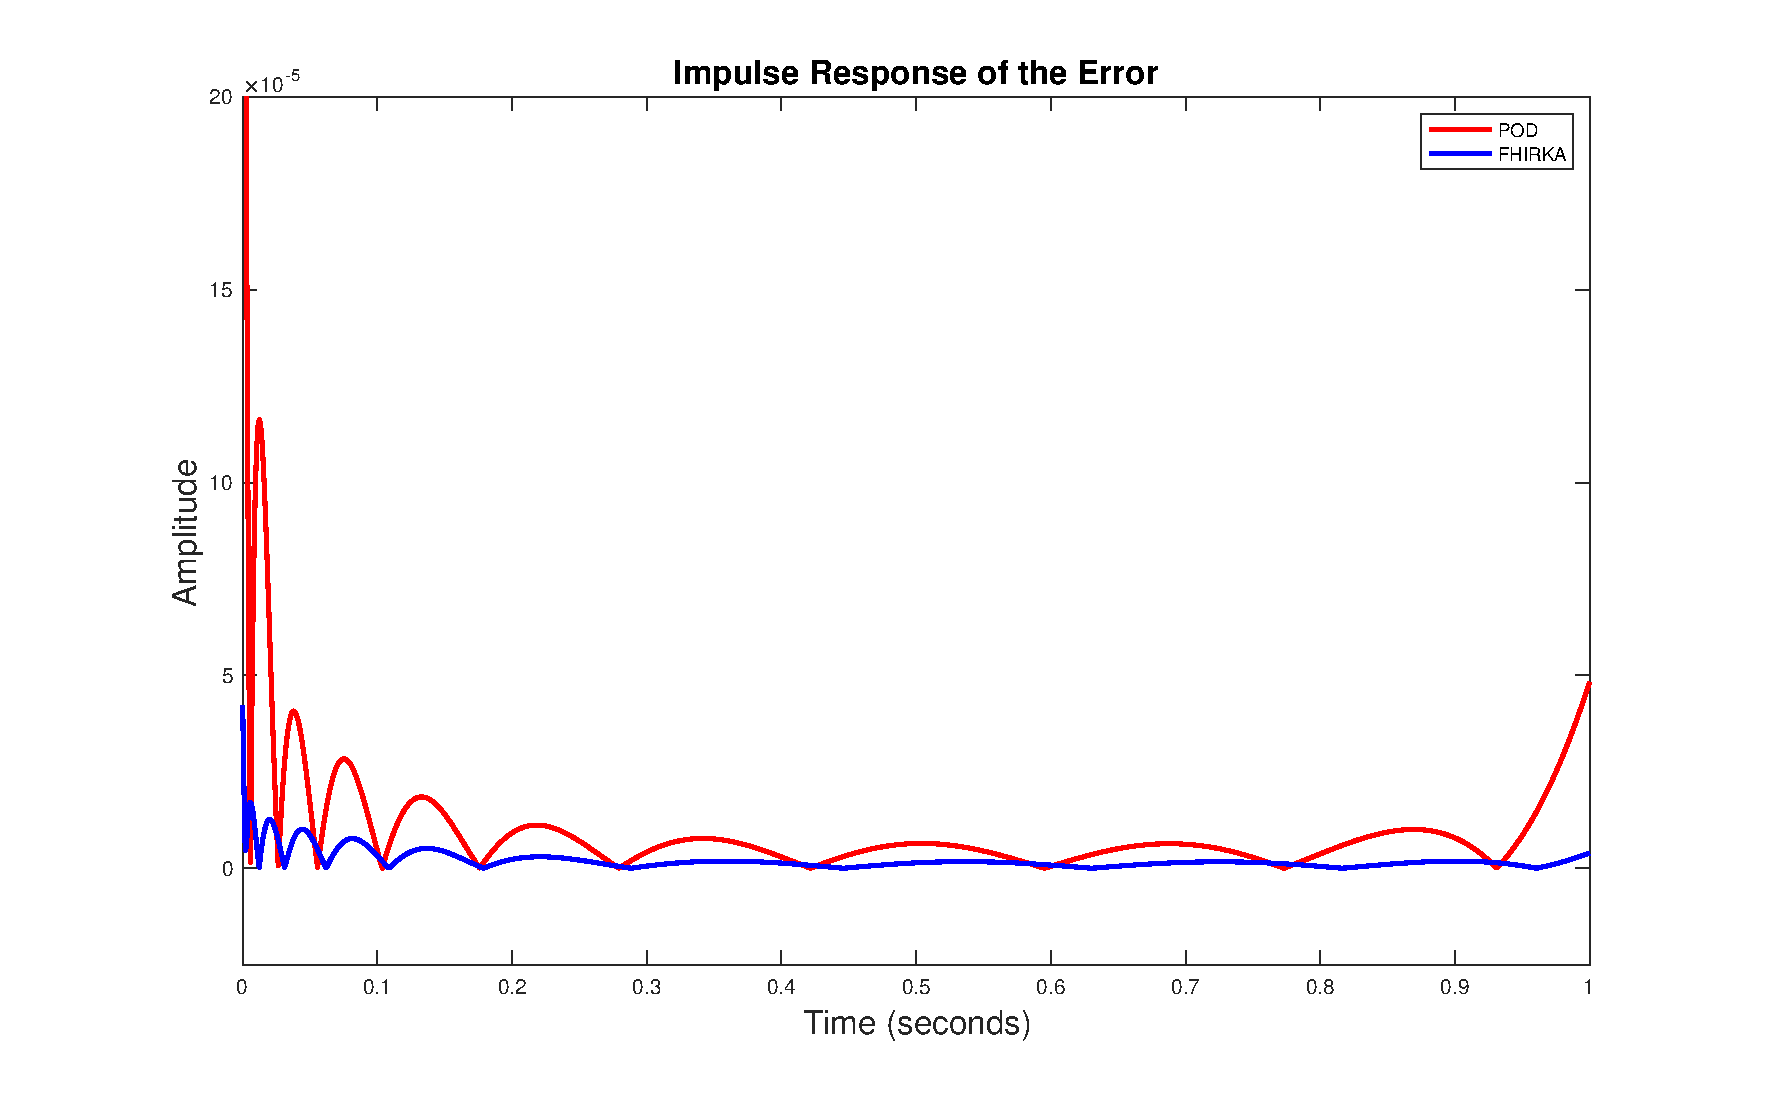
\includegraphics [scale=0.5]{absHeatErrorYlim}
      \caption{POD vs \FH for a heat model\label{fig:impulseHeat}}
 \end{figure}
 \begin{figure}[H]
 \centering
   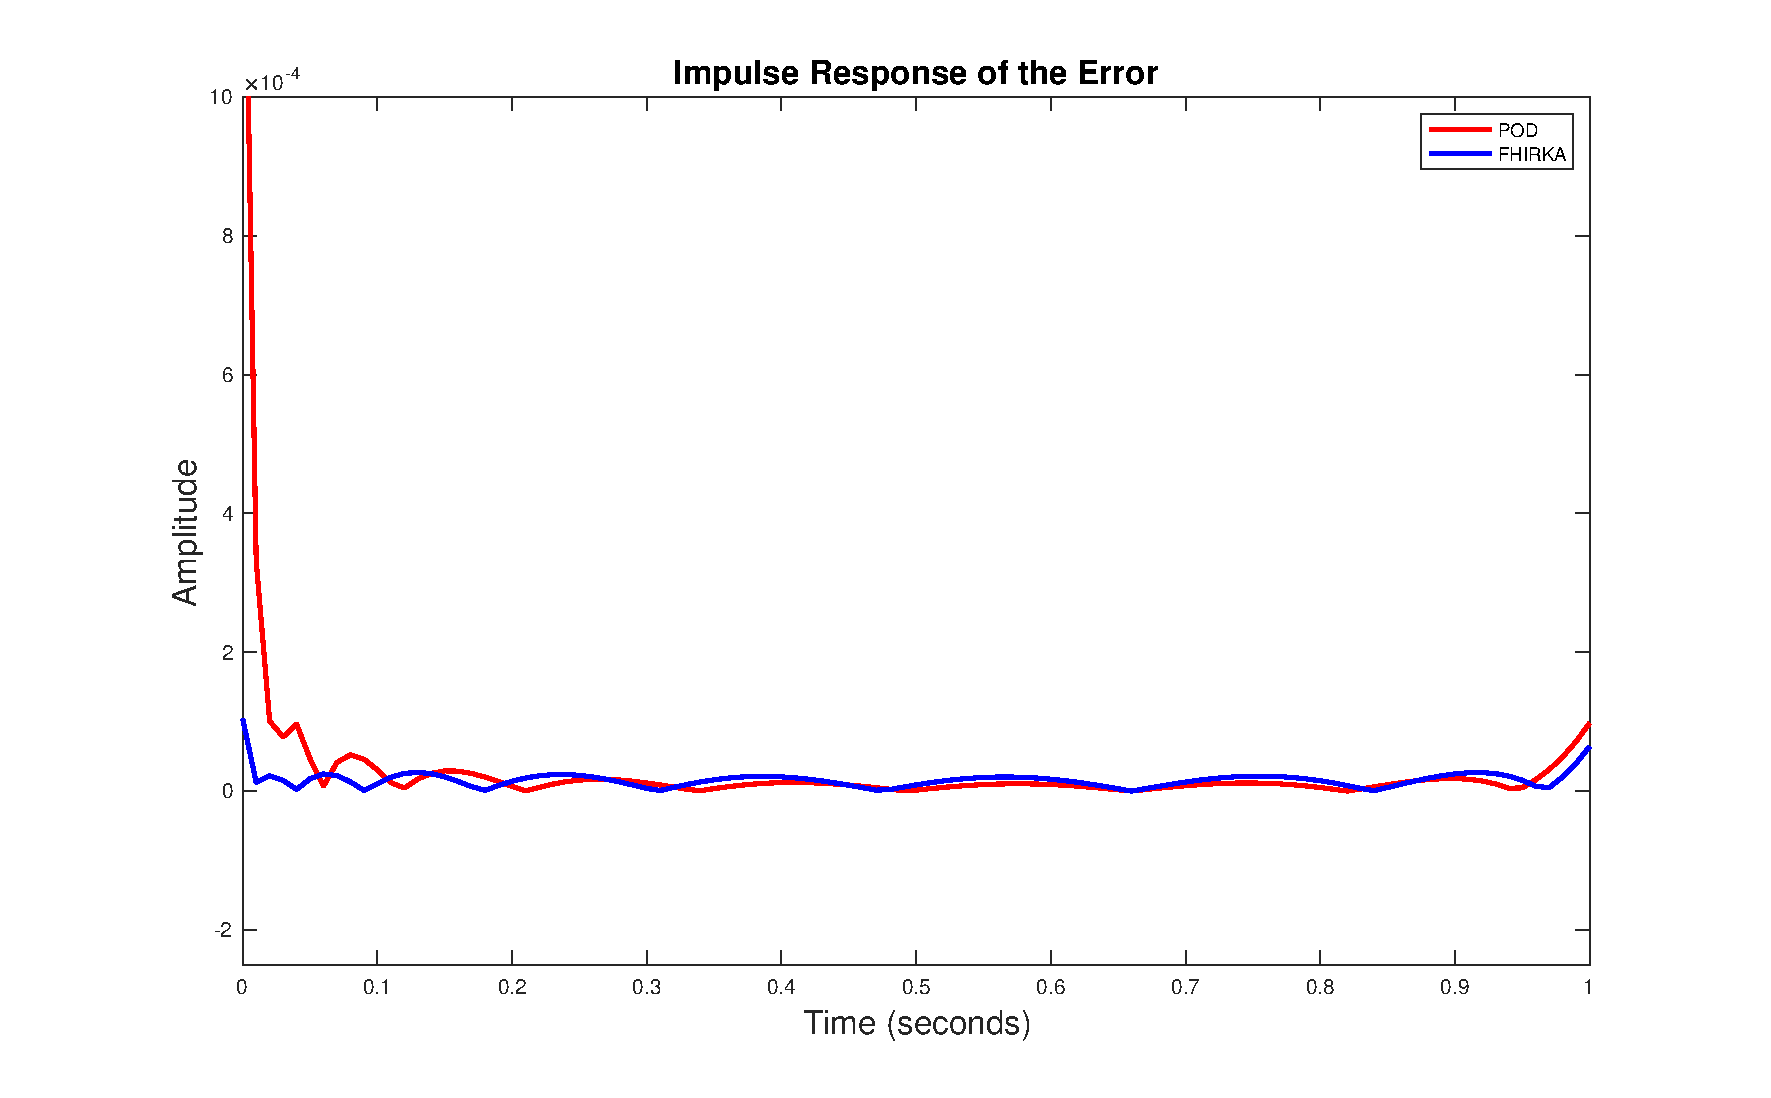
\includegraphics [scale=0.5]{absUNSError}
      \caption{POD vs \FH for an unstable model\ \label{fig:impulseUns}}
 \end{figure}



\item  There are some typos in the manuscript.  For example, the statement
"G(s) and Gr(s) be as defined in (3.5) and (3.5)" in Lemma 3.3 should
be corrected. \\
\serkan{\textsf{AR}:  We thank the referee for pointing out this issue. We have addressed it in the revised version.}

\end{itemize}

\end{document}